
\begin{frame}
[plain]
  \titlepage
\end{frame}


\begin{frame}{Human "Interactome"}
        \begin{center}
%        \setlength{\fboxsep}{0pt}
%          \fcolorbox{black}{white}{%
          \includegraphics[width=0.6\textwidth,trim={0 0 0cm 0},clip]{Human_interactome.jpg}
%           }
        \end{center}
\end{frame}

\begin{frame}{Особености белок-белковых контактов}
    \begin{itemize}
        \item Поверхность интерфейса большая, 1000-2000 \AA\tss{2} 
        \item Только 5\% остатков дают ключевой вклад в связывание
        \item Экспериментальный поиск затруднен
        \item Широкое разнообразие
        \end{itemize}
    \end{frame}

\begin{frame}{Способы предсказания белок-белковых взаимодействий}
    Взаимодействующие белки возможно ко-эволюционируют.
    \begin{itemize}
        \item Филогенетический профайлинг.\\
            Поиск пар белковых семейств среди широкого ряда видов. Появление и исчезновение пар семейств возможно
            указывает на взаимодействие.

        \item Предсказание на основе подобия филогенетических деревьев.
        \item Методы на основе классификации.
        \item Поиск гомологичных  мест контакта.
        \item Ассоциативные методы. Это поиск характеристических  последовательностей на основе профилей и мотивов.
    \end{itemize}
\end{frame}

\begin{frame}{Способы предсказания белок-белковых взаимодействий}
  %    \vspace{1cm}
    \begin{itemize}
        \item Идентификация структурных паттернов на основе известных структурных данных. \\
            Построение библиотеки и сканирование по ней.
        \item Методы Байеса для анализа экспериментальных результатов с значимым уровнем шума.
        \item Методы исключения доменных  пар. 
        \item Моделирование структуры комплекса на основе известной структуры и оценка его качества.
        \item Макромолекулярный докинг. 
    \end{itemize}
\end{frame}

  \begin{frame}{Базы данных}
      \begin{itemize}
          \item \textbf{String} - база данных экспериментальных и предсказанных  взаимодействий; отличная графика;
              http://string-db.org/
          \item \textbf{IntAct} - база данных  на основе литературных  данных или прямая информация от авторов.
              http://www.ebi.ac.uk/intact/
          \item \textbf{iHOP} - Информация слинкованая с другими белками. Построена на основе литературных  данных.
              Представление в виде кусочков текста. http://www.ihop-net.org/
          \item \textbf{BioGRID} - Источники: литература и результаты high-throughput экспериментов; 
              http://thebiogrid.org/
          \item \textbf{MIPS}   Mammalian Protein-Protein Interaction Database, не работает :). 
              http://mips.helmholtz-muenchen.de/proj/ppi
      \end{itemize}
  \end{frame}

\section{Макромолекулярный докинг}
\begin{frame}{Поиск наименьшего $\Delta G$}

    \begin{itemize}
        \item   Суть метода основывается на поиске соответствия поверхностей для достижения максимальной поверхности контакта.
        \item После нахождения возможных конфигураций происходит ранжирование.
            \begin{center}
%%        \setlength{\fboxsep}{0pt}
%          \fcolorbox{black}{white}{%
          \includegraphics[width=0.5\textwidth]{d1.eps}
%           } 

            \end{center}
        \end{itemize}
  \end{frame}

  \begin{frame}{Белковый докинг с использованием FFT}
            \begin{center}
%        \setlength{\fboxsep}{0pt}
%          \fcolorbox{black}{white}{%
          \includegraphics[width=0.8\textwidth]{fft.pdf}
 %          } 

            \end{center}
  \end{frame}

  \begin{frame}{Оценка производительности}
      \begin{itemize}
          \item Success Rate: для данного количества предсказаний ($N_p$), это процент структур для которых был найден
              как минимум один удачный результат
          \item Hit Count: среднее количество хитов при данном значении $N_p$.
      \end{itemize}
  \end{frame}


  \begin{frame}{Зависимость Success Rate от шага вращения}
            \begin{center}
%        \setlength{\fboxsep}{0pt}
%          \fcolorbox{black}{white}{%
          \includegraphics[width=0.7\textwidth]{step.pdf}
%           } 

            \end{center}
  \end{frame}


  \begin{frame}{Зависимость Hint count от шага вращения}
            \begin{center}
%        \setlength{\fboxsep}{0pt}
%          \fcolorbox{black}{white}{%
          \includegraphics[width=0.7\textwidth]{hc.pdf}
%           } 

            \end{center}
  \end{frame}

  \begin{frame}{Решеточная комплементарность поверхности}
            \begin{center}
%        \setlength{\fboxsep}{0pt}
%          \fcolorbox{black}{white}{%
          \includegraphics[width=0.7\textwidth]{gsc.pdf}
%           } 

            \end{center}
  \end{frame}


  \begin{frame}{Парная комплементарность поверхности}
            \begin{center}
%        \setlength{\fboxsep}{0pt}
%          \fcolorbox{black}{white}{%
          \includegraphics[width=0.7\textwidth]{psc.pdf}
%           } 

            \end{center}
  \end{frame}



  \begin{frame}{ PSC vs. GSC и  Success Rate}
      \begin{center}
%        \setlength{\fboxsep}{0pt}
%          \fcolorbox{black}{white}{%
          \includegraphics[width=0.7\textwidth]{psc_vs_gsc.pdf}
%           } 

            \end{center}
  \end{frame}


  \begin{frame}{Почему так? }
      \begin{center}
%        \setlength{\fboxsep}{0pt}
%          \fcolorbox{black}{white}{%
          \includegraphics[width=0.7\textwidth]{reason.pdf}
%           } 

            \end{center}
  \end{frame}

  \begin{frame}{Функция оценки энергии связывания}

      \[ \Delta G = \Delta E_{VdW} + \Delta E_{el.}+ \Delta G_{desol} +\Delta G_{const} \]

      \begin{itemize}
          \item $\Delta E_{VdW}$ - это комплементарность поверхности
          \item $\Delta G_{desol}$ - это гидрофобика
          \item $\Delta E_{el.}$ - это электростатика
          \item $\Delta G_{const}$ - это изменение вращательной и прочих энтропий.
          \end{itemize}

          \[  \Delta G_{desol}= \sum_i \sum_j N_{ij}\Delta G_{ij} \]
      \end{frame}

      \begin{frame}{Влияние на Succes rate}
      \begin{center}
%        \setlength{\fboxsep}{0pt}
%          \fcolorbox{black}{white}{%
          \includegraphics[width=0.8\textwidth]{desol_el.pdf}
%           } 

            \end{center}

      \end{frame}
      \begin{frame}{Влияние на Hit Count}
      \begin{center}
%        \setlength{\fboxsep}{0pt}
%          \fcolorbox{black}{white}{%
          \includegraphics[width=0.8\textwidth]{hc_desol_el.pdf}
%           } 

            \end{center}

      \end{frame}


      
      \section{Rosetta}
      \begin{frame}{Rosettadock Алгоритм}
          \begin{tikzpicture}
              \node (1)    [draw,ultra thick, fill=red!50!white]    {Случайное расположение};
              \node (2)    [draw, fill=green!50!black,below = of 1 ]    {Докинг с низким разрешением};
              \node (3)    [draw, fill=blue!50!black,below = of 2]    {Докинг с высоким разрешением};
              \node (4) [draw, fill=black!50!white,below = of 3] {$10^5$};
              \node (5) [draw, fill=cyan!50!black,right= of 4 ] {Кластеризация};
              \node (6) [draw, fill=magenta!50!black,right= of 5] {Результат};
              \node (7) [draw, fill=yellow!50!black,right= of 2] {Фильтры};
              \draw[-] (1) -> (2.north);
              \draw[-] (2) |- (3.north);
              \draw[-] (3) |- (4.north);
              \draw[-] (4.east) |- (5.west);
              \draw[-] (5.east) |- (6.west);
              \draw[-] (2.east) |- (7.west);
              \draw[-] (7.south) |- (3.east);
              \draw[-] (7.north) |- (1.east);

          \end{tikzpicture}    
      \end{frame}
\begin{frame}{Поиск с низким разрешением}
          Особенности метода:
          \begin{itemize}
              \item Поиск методом Монте-Карло.
              \item Вращение и смещение белка как жесткого тела.
              \item Остаток белка представляется как атомы остова и средний
                  центроид представляет боковой радикал.
              \item Процедура старается воспроизвести физическую диффузию.
          \end{itemize}
  \centering       
  \begin{tikzpicture}%
   \node (2) at (4,2) {%
     \footnotesize
     %\setatomsep{1.7em}\setcrambond{0.2em}{}{}%
     \chemfig[atom sep=1.7em, cram width=0.2em]{H{_2}N-[1](-[2]-[1]-[3](=[4]O)-[1]O{^-})-[7]C(=[6]O)-[1]N
         (-[2]H)-[7](-[6](-[7])-[5])-[1]C(=[2]O)-[7]N(-[6]H)
          -[1](-[2]-[1]**6(------))-[7]C(=[6]O)-[1]OH}};
     \node (d1) at (3,3) {\ddisk{orange}{2}};   
     \node (d2) at (3.85,0.5) {\ddisk{orange}{2}};   
     \node (d3) at (5,2.5) {\ddisk{orange}{2}};   
  \end{tikzpicture}
\end{frame}




      

      \begin{frame}{Уточнение с высоким разрешением} 
          \begin{itemize}
              \item Из библиотеки ротамеров добавляются полноатомные боковые цепи
              \item Используется полноценная оценка энергии (ММ)
              \item Монте-Карло + оптимизация геометрии
              \item Циклическое использование оптимизации положения как твердого
                  тела и полноатомная оптимизация положения боковых радикалов
          \end{itemize}
      \end{frame}


      \begin{frame}{Rosettadock Алгоритм}
          \begin{tikzpicture}
              \node (1)    [draw,fill=red!50!white]    {Случайное расположение};
              \node (2)    [draw, fill=green!50!black,below = of 1 ]    {Докинг с низким разрешением};
              \node (3)    [draw, ultra thick, fill=blue!50!black,below = of 2]    {Докинг с высоким разрешением};
              \node (4) [draw, fill=black!50!white,below = of 3] {$10^5$};
              \node (5) [draw, fill=cyan!50!black,right= of 4 ] {Кластеризация};
              \node (6) [draw, fill=magenta!50!black,right= of 5] {Результат};
              \node (7) [draw, fill=yellow!50!black,right= of 2] {Фильтры};
              \draw[-] (1) -> (2.north);
              \draw[-] (2) |- (3.north);
              \draw[-] (3) |- (4.north);
              \draw[-] (4.east) |- (5.west);
              \draw[-] (5.east) |- (6.west);
              \draw[-] (2.east) |- (7.west);
              \draw[-] (7.south) |- (3.east);
              \draw[-] (7.north) |- (1.east);

          \end{tikzpicture}    
      \end{frame}

      \begin{frame}{Пример докинга лигнада}
          \includegraphics[width=\textwidth]{rosetta-dock}
      \end{frame}

      \begin{frame}{HADDOCK}
          \includegraphics[width=\textwidth]{haddock}
      \end{frame}


\section{ML подходы к PPI}

\begin{frame}{История}
    \begin{itemize}
        \item Первые работы в 2001 году
        \item Суть задачи: для двух данных  последовательностей предсказать взаимодействие
        \item Типы представлений: состав, доменный состав, мотивы, профили гидрофобности, геномные особености, филогенетические особености
    \end{itemize}
\end{frame}

\begin{frame}{Типы подходов}
    \begin{itemize}
        \item Обучение с учителем: NN, Баевские методы, SVM, RF,
        \item Кластеризация
    \end{itemize}
 \footnotesize     *Наборы представлений, не могут полностью охватить динамические и сложные явления, которые могут
однозначно идентифицировать истинные IPP
\end{frame}
	
\begin{frame}{Поиск "hot spots"}
    \centering
    \includegraphics[height=.75\textheight]{ppi-hot.png}\\
    \footnotesize  10.3390/molecules23102535 
\end{frame}

\begin{frame}{Достижения}
    \begin{itemize}
        \item Существенный прогресс, но есть еще "вызовы"
        \item ddG из экспериментов не унифицированно
        \item Малое наполнение данными
        \item Часто случается переобучение
        \item Предикторы 'hot spots'   используют последовательность и структурную информацию для представления, но 3D не используется полностью
        \item *Перспективным считается интеграция физических методов (докинг, МД) и ML
    \end{itemize}
\end{frame}

\begin{frame}{D-SCRIPT}
    \includegraphics[height=.75\textheight]{ppi-dscript.png}\\
    \footnotesize 10.1016/j.cels.2021.08.010
\end{frame}

\begin{frame}{D-SCRIPT, результат}
    \includegraphics[height=.75\textheight]{ppi-dscript-res}\\
    \footnotesize
    *When D-SCRIPT correctly predicts an interaction, its contact maps are significantly similar to the ground truth.
\end{frame}

\begin{frame}{MASIF}
    \includegraphics[width=.8\textwidth]{masif-1} \\
    MaSIF-site: классификатор, на входе  поверхность белка, на выходе  прогнозируемая оценка для каждой вершины поверхности на
вероятность участия в PPI
\end{frame}

\begin{frame}{MASIF, предсказание участков}
    \centering
    \includegraphics[width=.8\textwidth]{masif-ppi-1}

\end{frame}
        
\begin{frame}{MASIF, сравнение }
    \includegraphics[width=.8\textwidth]{masif-ppi-2}
    \begin{itemize}
        \item PSIVER -  Naïve Bayes classifier  (NBC) and a kernel density estimation method (KDE)
        \item SPIDER -  SAS метрика + MSA, 
    \end{itemize}
\end{frame}

\begin{frame}{MASIF, предсказание для "новых" белков }
    \centering
    \includegraphics[height=.75\textheight]{masif-ppi-art}\\
    \footnotesize *MaSIF-site clearly labels the interfaces of the designs
\end{frame}

\begin{frame}{Ultrafast scanning with MASIF}
    \includegraphics[width=.8\textwidth]{masif-ppi-scan}\\
    \footnotesize *MaSIF-search inverts the numerical features of one  protein partner (multiplied by −1), with the exception of hydropathy. 
\end{frame}

\begin{frame}{"FATALITY" or not?}
    \includegraphics[height=.75\textheight]{masif-ppi-perf}\\
*Moreover, all these methods could benefit from sequence evolutionary data to improve their predictive capabilities.
\end{frame}

\begin{frame}{Masif-seed}
    \centering
    \includegraphics[height=.85\textheight]{masif-seed}\\
\end{frame}


\begin{frame}{ColabFold}
    \centering
    \includegraphics[height=.8\textheight]{ppi-alfafold-ovch.png}\\
    \footnotesize 10.1101/2021.08.15.456425v1.full.pdf
\end{frame}



\begin{frame}{AlphaFold-Multimer}
    \begin{itemize}
        \item Модификации функции loss, чтобы учесть симметрию перестановок для идентичных  цепей
        \item Совмещение двух  MSA для индивидуальных  цепей для утилизаци генетической информации об контакте
        \item Новый способ выборки набора остатков для обучения
        \item Разные мелкие оптимизации
    \end{itemize}
    \footnotesize 10.1101/2021.10.04.463034v1
\end{frame}

\begin{frame}{AlphaFold-Multimer}
    \centering
    \includegraphics[height=.9\textheight]{ppi-alfafold-0}\\
\end{frame}

\begin{frame}{AlphaFold-Multimer}
    \centering
    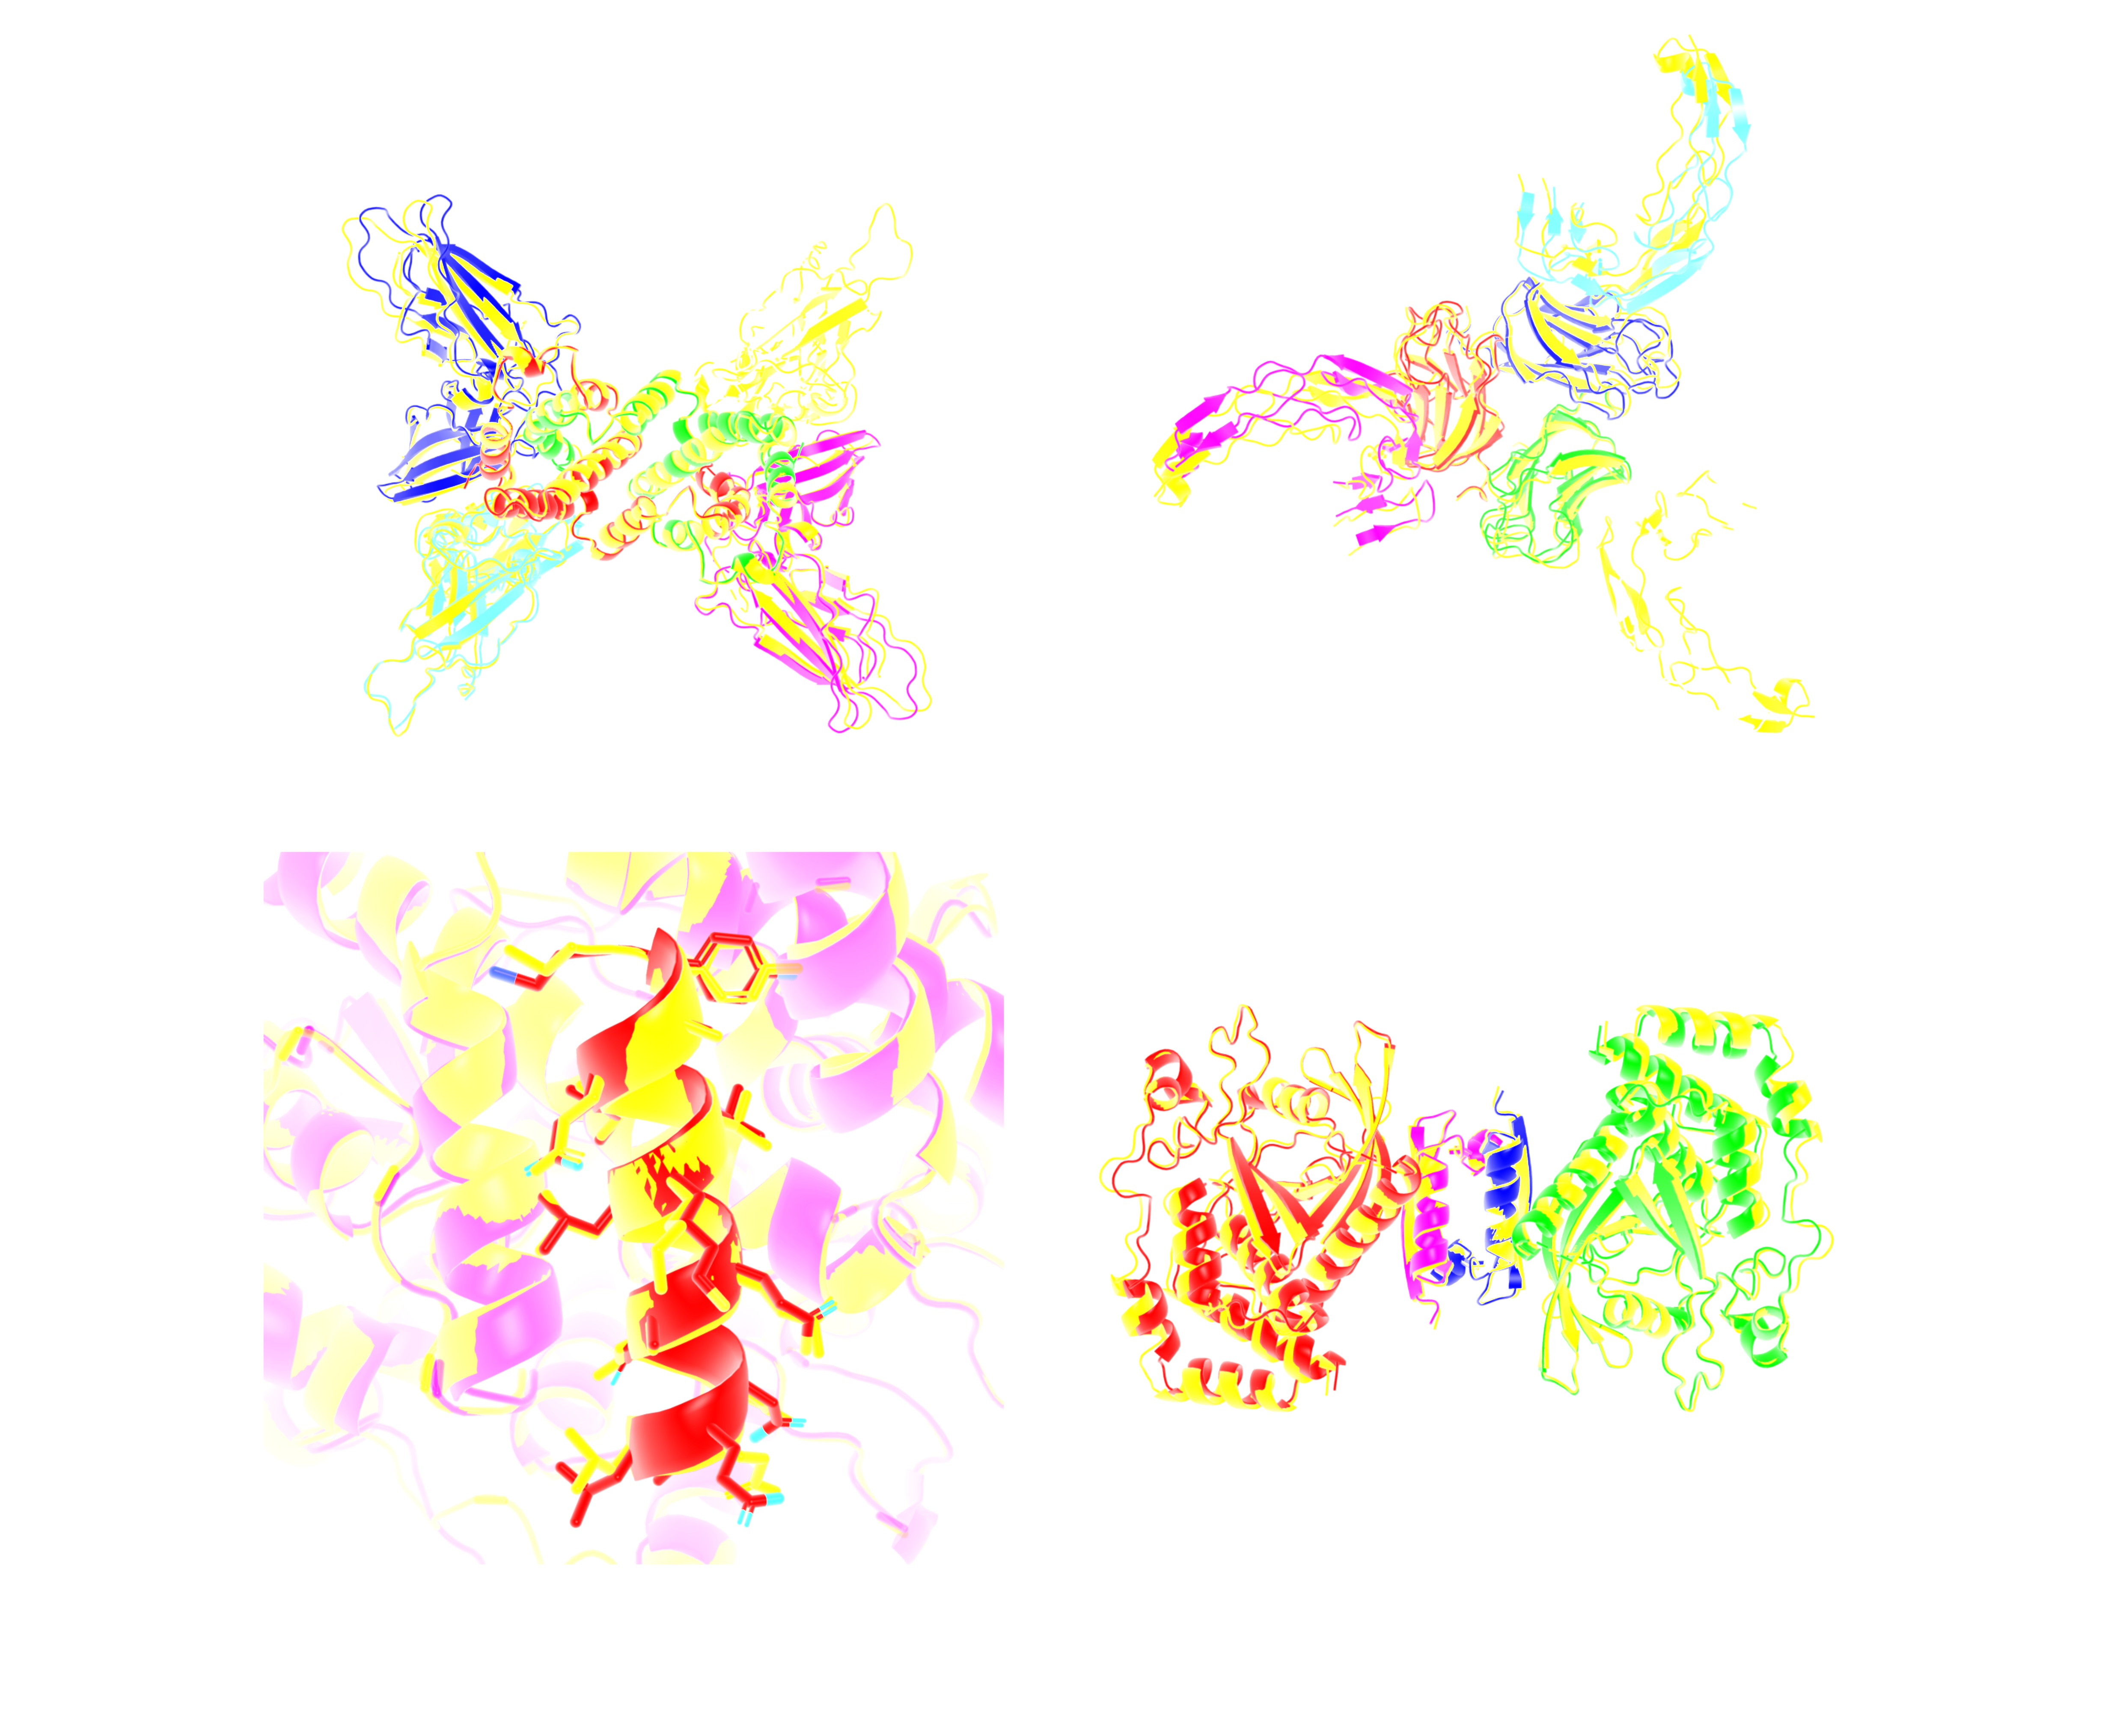
\includegraphics[height=.9\textheight]{ppi-alfafold-1}\\
\end{frame}

\begin{frame}{AlphaFold-Multimer}
    \centering
    \includegraphics[width=.9\textwidth]{ppi-alfafold-2}\\
\end{frame}



